% !TEX program = xelatex
% Đề thi cuối kỳ - Thiết kế và xây dựng phần mềm (20261)
% Gõ lại nguyên văn từ ảnh chụp đề 2.
\documentclass[11pt,a4paper]{article}
\usepackage{fontspec}
\setmainfont{Times New Roman}
\setsansfont{Arial}
\setmonofont{Consolas}
\usepackage[a4paper,top=1.0cm,bottom=1.0cm,left=1.9cm,right=1.9cm,headheight=0pt,headsep=0pt,footskip=18pt]{geometry}
\setlength{\emergencystretch}{2em}
\usepackage{enumitem}
\usepackage{amsmath}
\usepackage{amssymb}
\usepackage{graphicx}
\setlist[itemize]{topsep=0pt,partopsep=0pt,parsep=0pt,itemsep=1pt}
\setlist[enumerate]{topsep=0pt,partopsep=0pt,parsep=0pt,itemsep=0pt}
\usepackage{fancyhdr}
\pagestyle{fancy}
\fancyhf{}
\renewcommand{\headrulewidth}{0pt}
\fancyfoot[R]{\small Trang \thepage}%
\fancyfoot[L]{\scriptsize\itshape Lưu ý: sinh viên không được sử dụng tài liệu, điện thoại và máy tính}%
\linespread{1.0}
\setlength{\parindent}{0pt}
\setlength{\parskip}{2pt}
\newcommand{\cau}[2]{\par\vspace{2pt}\noindent\textbf{Câu #1.\ #2}\par\vspace{1pt}}
\newenvironment{pa}{\begin{list}{}{\leftmargin=0.95cm\labelwidth=0.5cm\labelsep=0.3cm\itemsep=1pt\parsep=0pt\topsep=0pt\partopsep=0pt}}{\end{list}}
\newcommand{\A}{\item[A.]}
\newcommand{\B}{\item[B.]}
\newcommand{\C}{\item[C.]}
\newcommand{\D}{\item[D.]}
\newcommand{\E}{\item[E.]}
\newcommand{\F}{\item[F.]}
\begin{document}

\noindent\textbf{Phần 1. (4 điểm) Trắc nghiệm, viết câu trả lời vào trong bài làm}

\cau{1}{Vì sao Analysis và Design được nói là ``không phải top-down cũng không phải bottom-up''?}
\begin{pa}
\A {\bfseries Vì use case đi vào từ giữa, định nghĩa một mức trung gian (middle level); từ đó có thể đi lên (subsystem) hoặc đi xuống (design class)}
\B Vì luôn bắt đầu từ design class rồi đi lên subsystem
\C Vì luôn bắt đầu từ subsystem rồi đi xuống design class
\D Vì analysis class được định nghĩa hoàn toàn theo hướng top-down
\end{pa}

\cau{2}{Khi chuyển đổi từ Analysis Classes sang Design Elements, mối quan hệ ánh xạ giữa chúng có đặc điểm gì? Chọn các phát biểu đúng.}
\begin{pa}
\A Một analysis class luôn ánh xạ đúng một design class tương ứng
\B {\bfseries Một analysis class có thể ánh xạ tới nhiều design elements khác nhau}
\C {\bfseries Nhiều analysis classes có thể cùng ánh xạ tới một design element}
\D Một analysis class loại \texttt{<<control>>} chỉ có thể ánh xạ tới một subsystem duy nhất
\E Một analysis class loại \texttt{<<entity>>} không thể trở thành một subsystem
\end{pa}

\cau{3}{Nhóm phát triển hệ thống quản lý bệnh viện xác định được analysis class \texttt{<<control>> TreatmentCoordinator} có các trách nhiệm sau: (1) điều phối quy trình khám chữa bệnh, (2) tính toán chi phí điều trị, (3) giao tiếp với hệ thống bảo hiểm bên ngoài, (4) lập lịch phòng mổ. Khi chuyển sang thiết kế, nhóm nên xử lý class này như thế nào? Chọn các phương án đúng.}
\begin{pa}
\A Giữ nguyên thành một design class vì đây là control class điều phối trung tâm
\B Gộp với class khác vì trách nhiệm của lớp này quá đơn giản
\C Chuyển toàn bộ thành một subsystem vì có giao tiếp với hệ thống ngoài
\D {\bfseries Tách phần giao tiếp với hệ thống bảo hiểm thành một interface riêng biệt}
\E {\bfseries Tách thành package chứa nhiều classes chuyên biệt để quản lý độ phức tạp}
\end{pa}

\cau{4}{Những phát biểu nào sau đây là đúng về vai trò của Subsystem so với Package?}
\begin{pa}
\A Cả subsystem và package đều cung cấp hành vi (behavior) cho hệ thống
\B {\bfseries Subsystem đóng gói hoàn toàn nội dung bên trong, trong khi package thì không}
\C {\bfseries Package dễ dàng thay thế hơn subsystem trong kiến trúc hệ thống}
\D {\bfseries Subsystem nâng cao mức độ trừu tượng hóa (level of abstraction) của hệ thống}
\E Subsystem và package đều có thể dễ dàng thay thế nhau mà không ảnh hưởng đến client
\end{pa}

\cau{5}{Nhóm phát triển ứng dụng quản lý bệnh viện đang thiết kế màn hình. Màn hình Danh sách bệnh nhân khi người dùng nhấn nút ``Xem chi tiết'' sẽ mở ra màn hình Hồ sơ bệnh nhân. Trong lúc xem hồ sơ, bác sĩ không thể quay lại thao tác trên danh sách cho đến khi đóng hồ sơ. Đây thuộc kiểu transition nào?}
\begin{pa}
\A {\bfseries Transition to a dependent child screen}
\B Simple screen transition
\C Transition to an independent child screen
\D Transition to a dependent screen
\end{pa}

\cau{6}{Theo chiến lược ``Defense in depth'', thứ tự đúng của bốn tầng phòng thủ chống lỗi (từ ưu tiên cao nhất đến thấp nhất) là:}
\begin{pa}
\A Debugging $\rightarrow$ Immediate visibility $\rightarrow$ Correctness $\rightarrow$ Impossible by design.
\B Correctness $\rightarrow$ Impossible by design $\rightarrow$ Debugging $\rightarrow$ Immediate visibility.
\C {\bfseries Impossible by design $\rightarrow$ Correctness $\rightarrow$ Immediate visibility $\rightarrow$ Debugging.}
\D Immediate visibility $\rightarrow$ Correctness $\rightarrow$ Debugging $\rightarrow$ Impossible by design.
\E Impossible by design $\rightarrow$ Immediate visibility $\rightarrow$ Correctness $\rightarrow$ Debugging.
\end{pa}

\cau{7}{Phát biểu nào đúng về quan hệ giữa độ phủ câu lệnh (C0) và độ phủ nhánh (C1) trong kiểm thử hộp trắng?}
\begin{pa}
\A C0 = 100\% luôn kéo theo C1 = 100\%.
\B {\bfseries Đạt C1 = 100\% luôn kéo theo C0 = 100\%.}
\C C0 và C1 hoàn toàn độc lập, không suy ra nhau.
\D Đạt C1 = 100\% đảm bảo module không còn lỗi.
\E C0 đo tỉ lệ nhánh đã được đi qua.
\F Đạt C1 = 100\% tương đương phủ hết mọi đường đi (path).
\end{pa}

\cau{8}{Bảng quyết định ``giao hàng nhanh'' của AMS Software với 3 điều kiện là C1: địa chỉ hỗ trợ, C2: có $\geq$1 sản phẩm hỗ trợ; C3: tất cả sản phẩm hỗ trợ. Tổ hợp nào bất khả thi (N/A)?}
\begin{pa}
\A C1=Y, C2=Y, C3=Y
\B C1=N, C2=Y, C3=N
\C C1=Y, C2=Y, C3=N
\D C1=N, C2=N, C3=N
\E C1=Y, C2=N, C3=N
\F {\bfseries C1=Y, C2=N, C3=Y}
\end{pa}

\cau{9}{Phát biểu nào về test oracle là đúng?}
\begin{pa}
\A Oracle là công cụ tự động sinh test case.
\B Oracle chỉ cần cho kiểm thử hộp trắng.
\C Khi dùng AI sinh test, oracle do AI đưa ra luôn đủ tin cậy.
\D {\bfseries Oracle là cơ chế xác định kết quả mong đợi để phán định pass/fail.}
\E Oracle và test case là cũng một khái niệm.
\end{pa}

\cau{10}{Điều gì phân biệt quan hệ phụ thuộc (dependency/identifying)\\ với quan hệ độc lập (independency/non-identifying) giữa quan hệ thực thể cha và con?}
\begin{pa}
\A Quan hệ phụ thuộc: khóa không dùng khóa ngoài.
\B {\bfseries Trong quan hệ phụ thuộc, khóa ngoài của con nằm trong khóa chính của con; trong quan hệ độc lập, khóa ngoài nằm ngoài khóa chính của con.}
\C Quan hệ phụ thuộc là 1-n, quan hệ độc lập là m-n.
\D Quan hệ phụ thuộc vẽ bằng nét đứt, quan hệ độc lập vẽ bằng nét liền.
\E Quan hệ phụ thuộc cho phép con tồn tại không cần cha, quan hệ độc lập thì không.
\end{pa}

\cau{11}{Mô hình dữ liệu khái niệm (conceptual data model, ví dụ E-R) có đặc điểm nào?}
\begin{pa}
\A {\bfseries Biểu diễn tự nhiên, độc lập với ràng buộc của DBMS cụ thể.}
\B Phụ thuộc vào DBMS cụ thể được chọn.
\C {\bfseries Là bước trước khi vẽ lược đồ quan hệ.}
\D Luôn ở dạng chuẩn 3NF.
\E Chỉ gồm bảng và khóa ngoài.
\F Dùng để mô tả chỉ số (index) và phân vùng lưu trữ.
\end{pa}

\cau{12}{Những phát biểu nào đúng về thiết kế lớp boundary?}
\begin{pa}
\A {\bfseries Hai lớp liên quan tới hai actor khác nhau.}
\B {\bfseries Một lớp optional và một lớp mandatory.}
\C {\bfseries Hai đối tượng trao đổi số lượng lớn message hoặc có giao tiếp phức tạp.}
\D Hai lớp hoàn toàn không có quan hệ nào với nhau.
\E {\bfseries Thay đổi hành vi của lớp này buộc phải thay đổi lớp kia.}
\F {\bfseries Loại bỏ một lớp làm lớp kia trở nên thừa.}
\end{pa}

\cau{13}{Những phát biểu nào cho thấy hai lớp có quan hệ chức năng (nên đặt chung package)?}
\begin{pa}
\A Hai lớp liên quan tới hai actor khác nhau.
\B Một lớp optional và một lớp mandatory.
\C {\bfseries Hai đối tượng trao đổi số lượng lớn message hoặc có giao tiếp phức tạp.}
\D Hai lớp hoàn toàn không có quan hệ nào với nhau.
\E {\bfseries Thay đổi hành vi của lớp này buộc phải thay đổi lớp kia.}
\F {\bfseries Loại bỏ một lớp làm lớp kia trở nên thừa.}
\end{pa}

\cau{14}{Khi thiết kế chữ ký operation, những ràng buộc nào là đúng?}
\begin{pa}
\A {\bfseries Càng ít tham số càng tốt, giúp tăng tính dễ hiểu và dễ bảo trì.}
\B {\bfseries Nên truyền nguyên cả đối tượng (ví dụ Student) thay vì truyền mảnh dữ liệu rời rạc.}
\C {\bfseries Nếu tham số không được sử dụng trong operation, nên thiết kế sao cho không được truyền nó.}
\D Càng nhiều tham số càng tốt.
\E {\bfseries Tránh by value nếu không cần.}
\F Không quan tâm tham số là optional hay có giá trị mặc định.
\end{pa}

\cau{15}{Những phát biểu đúng về navigability trong Class Design?}
\begin{pa}
\A Quan hệ hai chiều được chọn thay vì hai quan hệ một chiều.
\B {\bfseries Navigability được chọn theo nhu cầu sử dụng.}
\C {\bfseries Mặc dù association là hai chiều về mặt ngữ nghĩa, có thể chỉ cần thiết kế một chiều.}
\D {\bfseries Một mục tiêu của Design.}
\E Không có mối quan hệ nào cần mô hình.
\end{pa}

\cau{16}{Những phát biểu đúng về Generalization / Inheritance?}
\begin{pa}
\A Trong generalization, object của superclass có thể thay thế tùy ý cho object của subclass.
\B {\bfseries Generalization là quan hệ ``is a kind of'' và có tính bắc cầu (transitive).}
\C {\bfseries Subclass có thể dùng nơi superclass được dùng, nhưng không tùy ý ngược lại.}
\D {\bfseries ``Generalization'' là tên quan hệ, còn ``Inheritance'' là cơ chế hiện thực quan hệ đó.}
\E Multiple inheritance nghĩa là một superclass có nhiều subclass.
\end{pa}

\cau{17}{Những phát biểu nào đúng về so sánh quan hệ \texttt{<<include>>} và \texttt{<<extend>>}?}
\begin{pa}
\A {\bfseries Trong \texttt{<<include>>}, use case được include luôn luôn được thực thi.}
\B {\bfseries Trong \texttt{<<extend>>}, use case mở rộng chỉ được thực thi khi điều kiện mở rộng thỏa mãn.}
\C {\bfseries Base use case trong quan hệ \texttt{<<extend>>} là hành vi không có use case mở rộng.}
\D {\bfseries Base use case trong quan hệ \texttt{<<include>>} là use case luôn dùng chứa một use case khác.}
\E Chỉ phụ thuộc của \texttt{<<extend>>} là hành vi khác nhau.
\end{pa}

\cau{18}{Chọn tất cả các thiết kế dữ liệu vi phạm 1NF.}
\begin{pa}
\A {\bfseries Cột authors chứa ``Nguyễn A; Trần B; Lê C'' trong một ô.}
\B {\bfseries Cột tracklist lưu toàn bộ danh sách bài hát ngăn bằng dấu phẩy trong một ô.}
\C Mỗi dòng OrderMedia lưu đúng một (mediaId, quantity).
\D {\bfseries Cột phoneNumbers chứa nhiều số điện thoại trong cùng một ô.}
\E Tách bảng Author riêng và nối Book--Author qua bảng trung gian.
\F Lưu một địa chỉ của một người thành nhiều ô.
\end{pa}

\cau{19}{Lựa chọn nào là thực hành tốt khi đặc tả use case?}
\begin{pa}
\A {\bfseries Đặt tên use case bắt đầu bằng động từ (động từ + danh từ).}
\B Dùng các từ như ``màn hình'', ``cửa sổ'', ``ô nhập liệu'' để mô tả giao diện.
\C {\bfseries Đặt tên actor theo vai trò trong hệ thống.}
\D {\bfseries Mô tả các bước theo trình tự, không phụ thuộc vào giao diện cụ thể.}
\E {\bfseries Mỗi bước nên nêu rõ actor thực hiện và phản hồi của hệ thống.}
\end{pa}

\cau{20}{Phát biểu nào về gate trong interaction diagram là đúng?}
\begin{pa}
\A Gate là một lớp trung gian của subsystem.
\B Gate chỉ tồn tại trong sequence diagram.
\C {\bfseries Gate có thể truyền message vào hoặc ra khỏi một interaction.}
\D {\bfseries Gate là điểm kết nối cho một message đi vào hoặc đi ra khỏi một interaction.}
\end{pa}

\newpage
\noindent\textbf{Phần 2.} Bạn cần thiết kế và xây dựng một hệ thống đặt vé xem phim trực tuyến cho một hệ thống rạp chiếu phim có nhiều cụm rạp tại các thành phố khác nhau. Mỗi cụm rạp sở hữu nhiều phòng chiếu với sức chứa khác nhau: 60, 120 và 250 ghế.
\begin{itemize}[leftmargin=1.05cm]
\item Mỗi phòng chiếu được định danh bằng mã phòng và số hiệu cụm rạp để đảm bảo tính duy nhất. Các suất chiếu được vận hành theo lịch cố định trong ngày; mỗi phim được xếp vào các khung giờ xác định trước. Mỗi suất chiếu có một phim và một nhân viên vận hành chịu trách nhiệm. Với các phim dài, hệ thống cho phép có giờ nghỉ giữa chừng.
\item Hệ thống hỗ trợ hai loại suất chiếu để đáp ứng các nhu cầu khác nhau: \textbf{Suất chiếu thường}: Giá vé tiêu chuẩn, chiếu trên các phòng 2D thông thường, cho phép đặt mọi hạng ghế. \textbf{Suất chiếu đặc biệt (3D/IMAX)}: Giá vé cao hơn, chỉ chiếu trên các phòng kỹ thuật cao, bắt buộc đặt theo khu vực ghế.
\item Khách hàng có thể đăng ký tài khoản và thực hiện thanh toán trước qua thẻ tín dụng hoặc liên ngân hàng; hoặc thanh toán sau tại quầy. Nếu khách hủy vé, hệ thống hoàn lại 80\% giá trị vé. Tuy nhiên, không chấp nhận hủy vé trong vòng 2 giờ trước giờ chiếu. Các ghế được giải phóng sẽ được bán lại cho khách hàng khác. Vé chưa thanh toán sẽ bị hủy nếu khách hàng không có mặt 30 phút trước giờ chiếu.
\end{itemize}


\noindent\textbf{Trả lời các câu hỏi sau:}

\noindent a) (3 điểm) Xây dựng biểu đồ lớp (thiết kế) cho use case \textbf{``Đặt vé xem phim''} được mô tả như trên. Lưu ý: phần thiết kế của bạn không bao gồm use case được gói đến \textbf{``Thanh toán trực tuyến''}.

\par\nobreak\vspace*{0pt}
{\itshape\nobreak Luồng sự kiện chính:}
\begin{enumerate}[leftmargin=1.05cm]
\item Khách hàng truy cập tính năng đặt vé.
\item Hệ thống hiển thị danh sách các suất chiếu trong ngày hôm nay. Nếu suất chiếu đã bán hết hoặc đã bắt đầu thì không cho phép đặt vé.
\item Khách hàng chọn cụm rạp, tên phim, ngày chiếu và gửi yêu cầu tìm kiếm.
\item Hệ thống hiển thị các suất chiếu còn ghế trống cùng giờ chiếu (giờ:phút), loại phòng (60/120/250 ghế), giá vé và loại suất chiếu (thường / đặc biệt).
\item Khách hàng chọn suất chiếu.
\item Hệ thống hiển thị chi tiết suất chiếu: mã phòng, số hiệu cụm rạp, thông tin nhân viên vận hành, thời lượng và giờ kết thúc dự kiến; nếu là suất đặc biệt thì hiển thị sơ đồ khu vực ghế bắt buộc.
\item Khách hàng chọn số lượng và vị trí ghế, nhập thông tin liên hệ (họ tên, số điện thoại, email), xác nhận đặt vé.
\item Hệ thống tính toán và hiển thị chi tiết đặt vé: thông tin suất chiếu; số lượng ghế, hàng ghế, đơn giá, tổng tiền cần thanh toán; thông tin liên hệ khách hàng.
\item Khách hàng chọn hình thức thanh toán: trước qua thẻ tín dụng/ngân hàng (kết nối cổng thanh toán) hoặc sau (tại quầy).
\item Nếu chọn thanh toán trước, hệ thống gọi use case ``Thanh toán trực tuyến'' để xử lý giao dịch.
\item Sau khi hoàn tất, hệ thống gửi thông báo xác nhận và hiển thị thông tin đặt vé thành công.
\item Nếu đã thanh toán trước, hệ thống cung cấp vé điện tử (mã đặt chỗ) qua email hoặc SMS.
\end{enumerate}
\par\nobreak\vspace{0pt}
{\itshape\nobreak Luồng sự kiện thay thế:}
\begin{itemize}[leftmargin=1.05cm]
\item Nếu khách hàng nhập sai thông tin, hệ thống hiển thị thông báo lỗi và yêu cầu nhập lại.
\item Nếu không có suất chiếu nào phù hợp, hệ thống thông báo và đề xuất ngày/suất khác nếu có.
\item Nếu thanh toán trực tuyến thất bại, hệ thống yêu cầu khách hàng thử lại hoặc chọn phương thức khác.
\end{itemize}

\par\vspace{3pt}
\noindent b) (1 điểm) Trên biểu đồ lớp đã thiết kế ở câu a), xét nhận định sau: \textit{«lớp Đặt vé vừa tìm suất chiếu còn trống, vừa tính tiền vé, vừa gọi cổng thanh toán, vừa gửi email/SMS xác nhận cho khách.»} Nhận định trên phản ánh vấn đề về \textbf{độ kết dính (cohesion)} hay \textbf{độ ghép nối (coupling)}? Hãy gọi tên cụ thể mức/loại và giải thích ngắn gọn vì sao. Chỉ ra lớp (hoặc quan hệ giữa các lớp) trong thiết kế của bạn đang gặp vấn đề này. Đề xuất hướng tái cấu trúc để khắc phục (tăng cohesion / giảm coupling), nêu rõ kết quả mong đợi sau khi sửa.

\par\vspace{3pt}
\noindent c) (2 điểm) Hãy đánh giá \textbf{bản thiết kế} của bạn trong câu \textbf{a} (có vi phạm nguyên lý thiết kế \textbf{SOLID} nào không) khi trong tương lai có thể gặp các tình huống thay đổi / phát sinh sau. Với mỗi tình huống, nếu thiết kế của bạn chưa tốt thì cần chỉ ra rõ ràng và đưa ra định hướng giải pháp
\begin{itemize}[leftmargin=1.05cm,itemsep=0pt]
\item Hệ thống có thêm các phòng chiếu với sức chứa khác, ví dụ 40 hoặc 180 ghế.
\item Hệ thống có thêm các loại phòng khác như phòng Gold Class / Beanbag với ghế nằm rộng và tiện nghi hơn so với phòng thông thường.
\item Giá vé phụ thuộc vào từng loại phòng, như phòng Gold Class sẽ đắt hơn phòng thông thường.
\item Hệ thống có thêm các hình thức thanh toán khác như Momo, ZaloPay, Apple Pay...
\end{itemize}

\newpage
\begin{center}
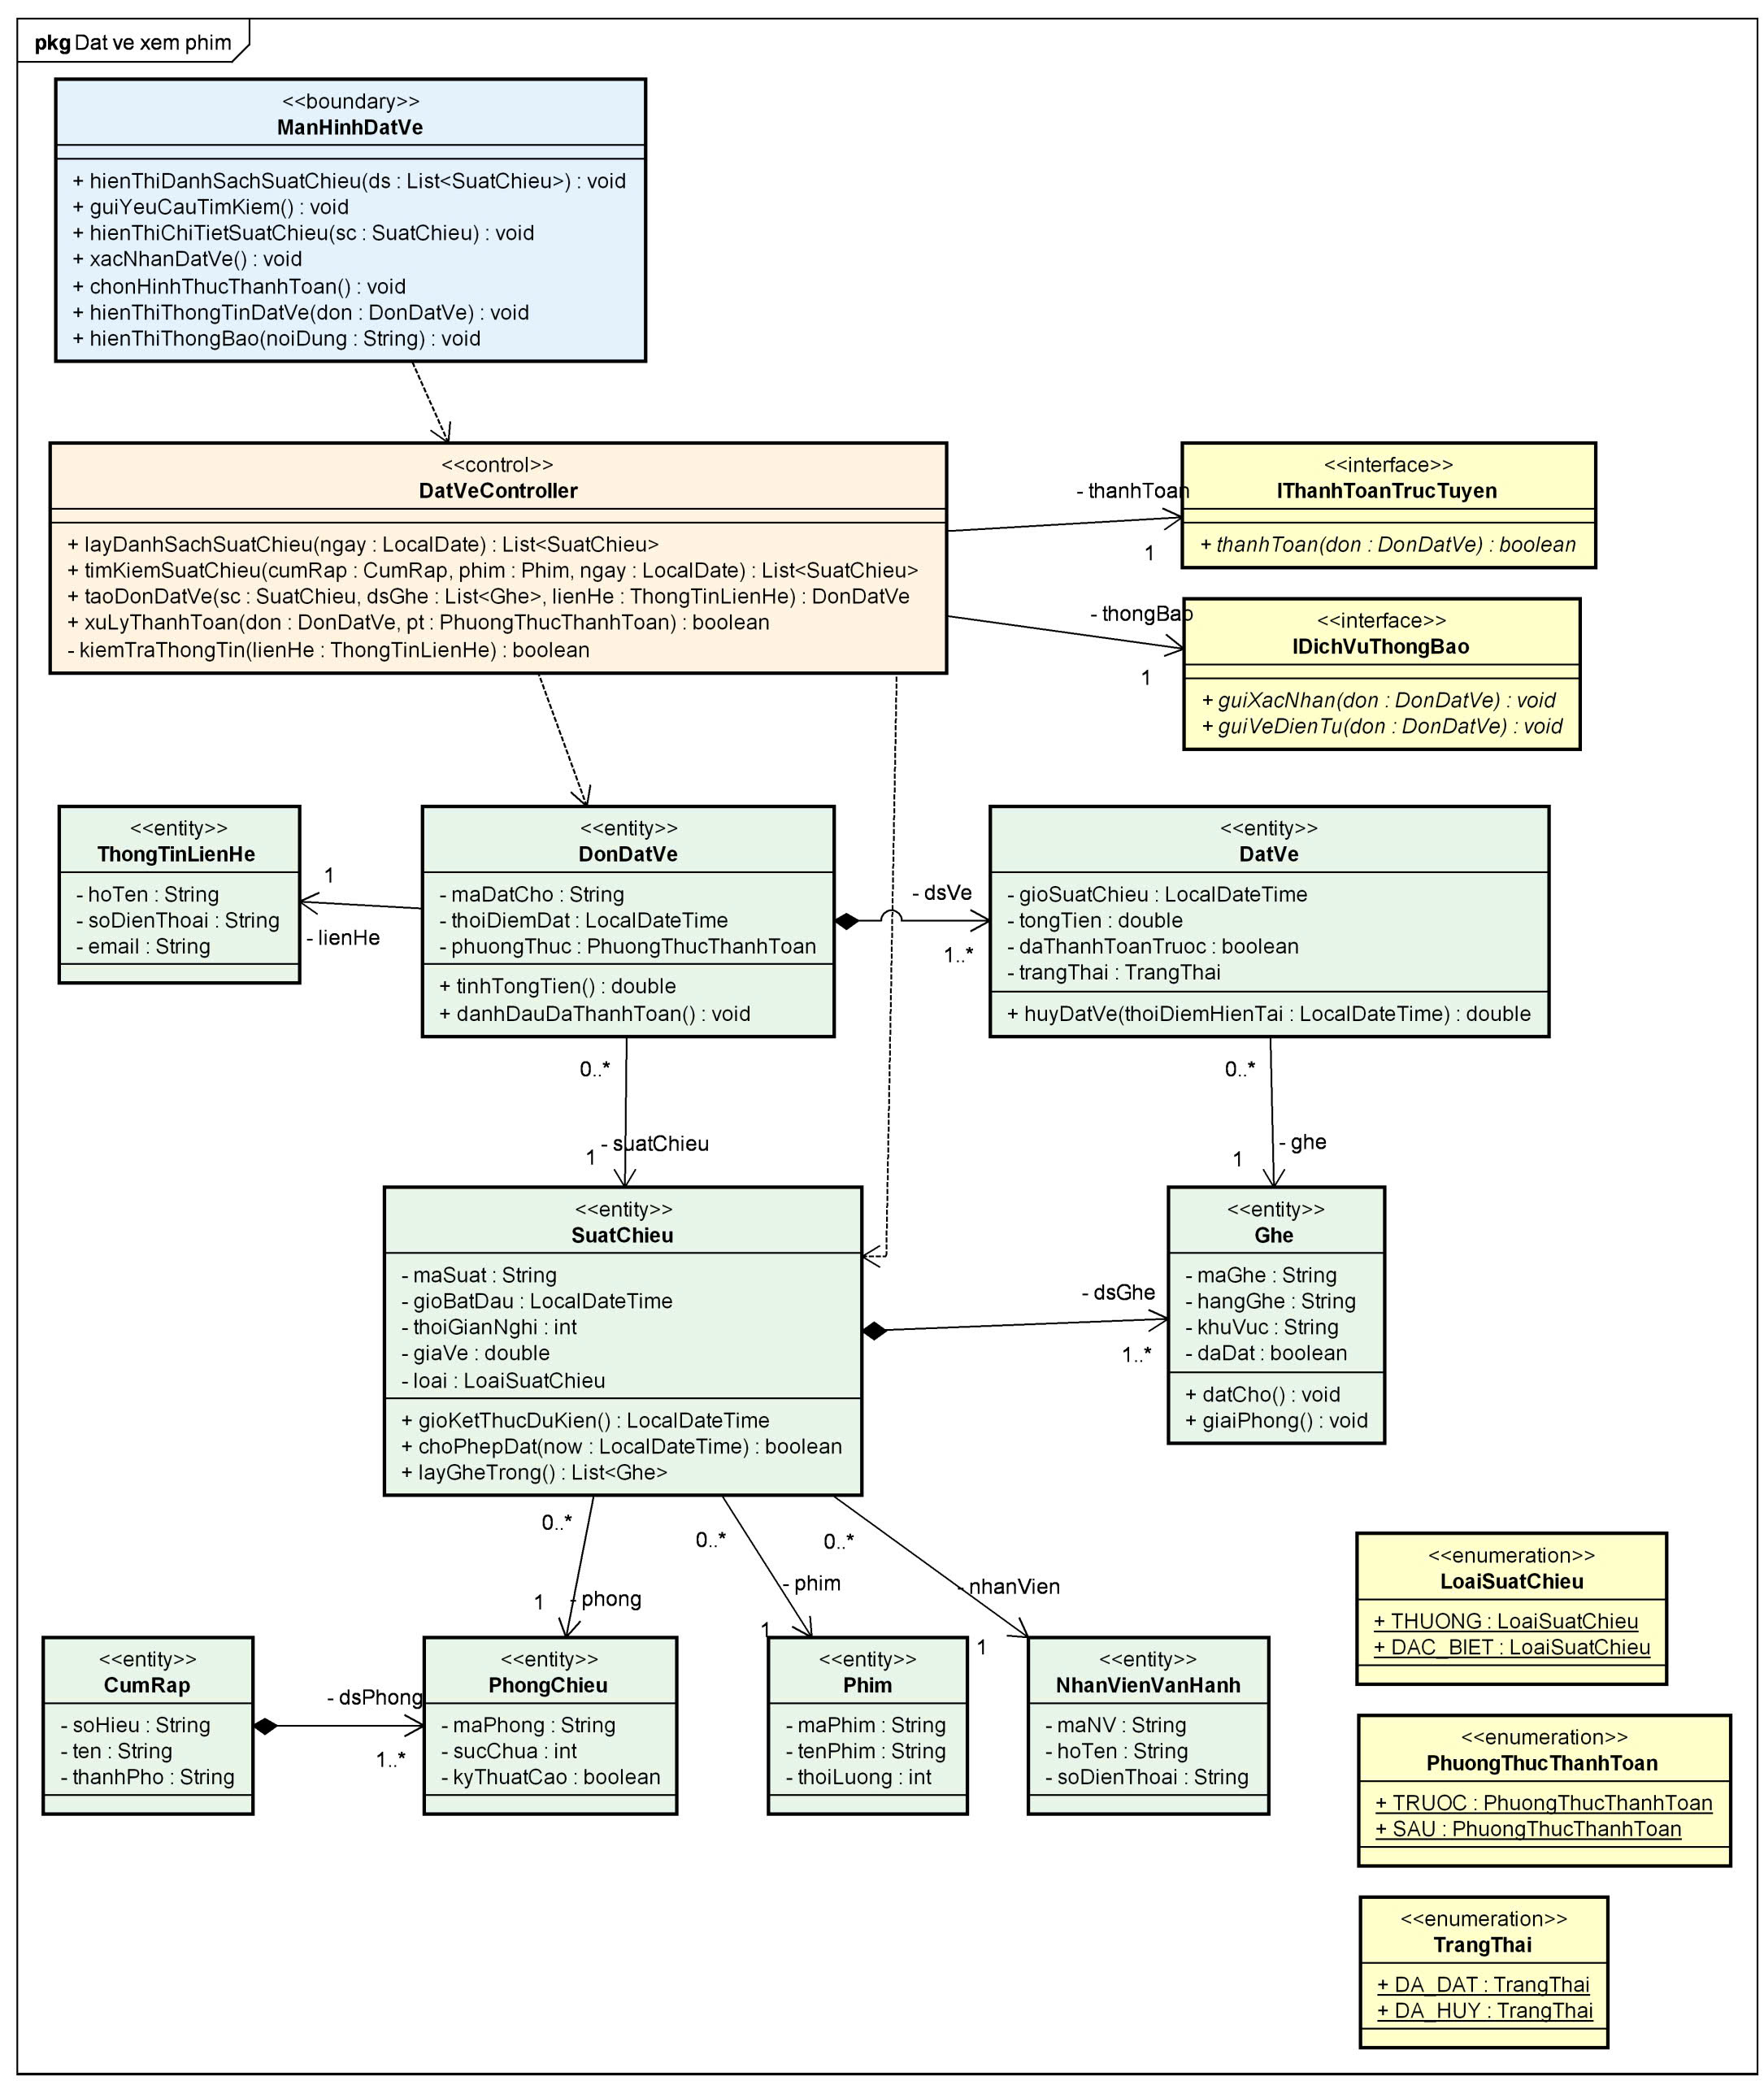
\includegraphics[width=\textwidth,height=0.96\textheight,keepaspectratio]{_images/de2_p5.jpg}
\end{center}


\newpage
\section*{ĐÁP ÁN VÀ LỜI GIẢI THAM KHẢO}
\subsection*{Phần 1 -- Đáp án trắc nghiệm}
{\setlength{\tabcolsep}{3pt}
\begin{tabular}{llllll}
Câu 1: \textbf{A} & Câu 2: \textbf{B,C} & Câu 3: \textbf{D,E} & Câu 4: \textbf{B,C,D} & Câu 5: \textbf{A} & Câu 6: \textbf{C}\\
Câu 7: \textbf{B} & Câu 8: \textbf{F} & Câu 9: \textbf{D} & Câu 10: \textbf{B} & Câu 11: \textbf{A,C} & Câu 12: \textbf{A,B,C,E,F}\\
Câu 13: \textbf{C,E,F} & Câu 14: \textbf{A,B,C,E} & Câu 15: \textbf{B,C,D} & Câu 16: \textbf{B,C,D} & Câu 17: \textbf{A,B,C,D} & Câu 18: \textbf{A,B,D}\\
Câu 19: \textbf{A,C,D,E} & Câu 20: \textbf{C,D} & & & &
\end{tabular}}

\subsection*{Phần 2 -- Lời giải tự luận}
\textbf{a) Thiết kế lớp cho use case ``Đặt vé xem phim''.}

Thiết kế đề xuất gồm: \textbf{Customer}; \textbf{CinemaComplex} chứa nhiều \textbf{ScreeningRoom}; \textbf{ScreeningRoom} có roomId, roomNumber, roomType, capacity và các \textbf{Seat}; \textbf{Movie}; \textbf{Screening} gắn Movie, ScreeningRoom, start/end time và Employee vận hành; \textbf{Booking} gắn Customer và Screening, chứa nhiều \textbf{BookingItem/Ticket} (seat, seat type, unit price, trạng thái). Các lớp service/interface gồm ScreeningSearchService, SeatAvailabilityService (kiểm tra và giữ ghế có thời hạn), PricingService, PaymentService và NotificationService. BookingController hoặc ReservationService chỉ điều phối luồng.

Luồng xử lý là tìm suất còn chỗ theo cụm rạp/phim/ngày; kiểm tra suất chưa bắt đầu; chọn ghế và giữ ghế; tính tiền và tạo Booking; nếu thanh toán trước thì gọi PaymentService (chi tiết use case thanh toán trực tuyến nằm ngoài phạm vi); sau khi thành công gửi thông báo và cấp mã đặt chỗ. Việc kiểm tra ghế phải thực hiện lại tại thời điểm xác nhận để chống đặt trùng. Capacity, room type, seat map và giá là dữ liệu/chính sách cấu hình, không hard-code trong controller.

\textbf{b) Cohesion/coupling.} Câu mô tả ``lớp Đặt vé'' có \textbf{cohesion thấp}: một lớp gánh các trách nhiệm khác bản chất (tìm suất, tính tiền, thanh toán, thông báo), gần với logical/coincidental cohesion thay vì functional cohesion. Nó cũng tạo \textbf{coupling cao} với cổng thanh toán và kênh thông báo. Tách các service/interface chuyên trách, dùng dependency injection và adapter cho hệ thống ngoài sẽ tăng cohesion của từng lớp, giảm coupling của ReservationService, đồng thời thuận lợi cho kiểm thử và thay thế nhà cung cấp.

\textbf{c) Đánh giá SOLID.}
\begin{itemize}[leftmargin=1.05cm,itemsep=1pt]
  \item Phòng 40/180 ghế: tránh if/else theo danh sách cố định; capacity và seat map thuộc cấu hình ScreeningRoom. Đây là cách tuân thủ OCP và SRP.
  \item Gold Class/Beanbag: biểu diễn RoomType/SeatType hoặc abstraction về đặc tính phòng; không ép mọi phòng phải có hành vi/thuộc tính không phù hợp. Các implementation phải thay thế được abstraction (LSP).
  \item Giá theo phòng: đưa quy tắc vào PricingPolicy/Strategy, chẳng hạn StandardPricing và PremiumRoomPricing. ReservationService chỉ phụ thuộc PricingService, không tự biết bảng giá (SRP/OCP/DIP).
  \item Momo/ZaloPay/Apple Pay: tạo PaymentGateway interface và adapter cho từng provider. Inject abstraction vào PaymentService; thêm provider mới không sửa controller hay logic đặt vé (DIP/OCP).
\end{itemize}

\textbf{Kết luận:} một controller mỏng, entity có trách nhiệm miền vừa phải và các service chuyên trách tạo ra functional cohesion cao hơn; các interface ngăn phụ thuộc trực tiếp vào chi tiết triển khai và giữ thiết kế mở cho mở rộng.

\end{document}
